\documentclass[a4paper]{article}
\usepackage{amsmath}

\usepackage{tikz}
\usetikzlibrary{matrix,calc,positioning}

\begin{document}

\tikzstyle{column 1}=[nodes={minimum width=4cm}]


\centering

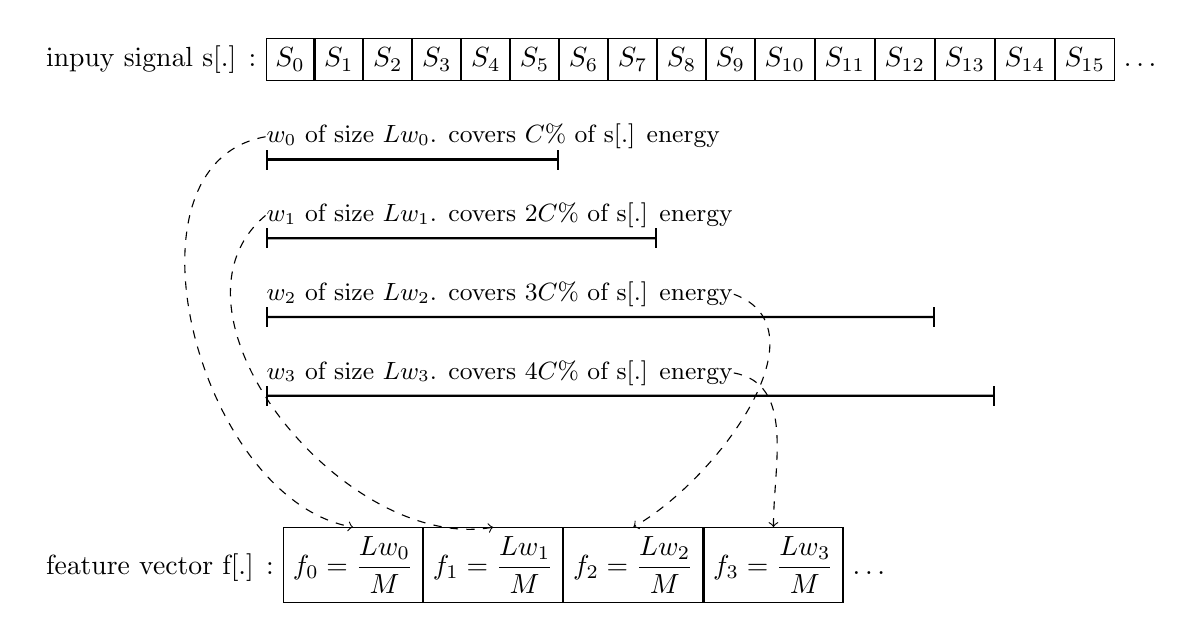
\begin{tikzpicture}[row 1/.style={nodes={draw}},node distance=6cm]
\matrix(M)[matrix of nodes]
{
|[draw=none]|inpuy signal s[.] :& $S_0$ & $S_1$ & $S_2$ & $S_3$ & $S_4$ & $S_5$ & $S_6$ & $S_7$ & $S_8$ & $S_9$ & $S_{10}$ & $S_{11}$ & $S_{12}$ & $S_{13}$ & $S_{14}$ & $S_{15}$ & |[draw=none]| $\ldots$ \\
};


\draw[|-|,thick]($(M-1-2.south west)+(0,-1cm)$)--($(M-1-7.south east)+(0,-1)$)node (A) [above,pos=0,anchor=south west,inner xsep=0pt,font=\small]{$w_0$ of size $Lw_0$. covers $C\%$ of s[.] energy};
\draw[|-|,thick]($(M-1-2.south west)+(0,-2cm)$)--($(M-1-9.south east)+(0,-2)$)node (B) [above,pos=0,anchor=south west,inner xsep=0pt,font=\small]{$w_1$ of size $Lw_1$. covers $2C\%$ of s[.] energy};
\draw[|-|,thick]($(M-1-2.south west)+(0,-3cm)$)--($(M-1-14.south east)+(0,-3)$)node (C) [above,pos=0,anchor=south west,inner xsep=0pt,font=\small]{$w_2$ of size $Lw_2$. covers $3C\%$ of s[.] energy};
\draw[|-|,thick]($(M-1-2.south west)+(0,-4cm)$)--($(M-1-15.south east)+(0,-4)$)node (D) [above,pos=0,anchor=south west,inner xsep=0pt,font=\small]{$w_3$ of size $Lw_3$. covers $4C\%$ of s[.] energy};

\matrix(L) [matrix of nodes, below= of M.south west,anchor=west]
{
|[draw=none]|feature vector f[.] :& $f_0=\dfrac{Lw_0}{M}$ & $f_1=\dfrac{Lw_1}{M}$ & $f_2=\dfrac{Lw_2}{M}$ & $f_3=\dfrac{Lw_3}{M}$ & |[draw=none]| $\ldots$ \\
};

\draw[dashed,->](A.west) to [out=190,in=170](L-1-2.north);
\draw[dashed,->](B.west) to [out=220,in=190](L-1-3.north);
\draw[dashed,->](C.east) to [out=-20,in=30](L-1-4.north);
\draw[dashed,->](D.east) to [out=-10,in=90](L-1-5.north);
\end{tikzpicture}

\end{document}
